%%%%%%%%%%%%%%%%%%%%%%%%%%%%%%%%%%%%%%%%%%%%%%%%%%%%%%%%%%%%%%%%%%%%%%%%%%%%%%%%%%%%%%%%%%%%%%%%%%%%%%%
% PACKAGES

\documentclass[a4paper, 11pt]{article}
\usepackage[utf8]{inputenc}
\usepackage[T1]{fontenc}
%\usepackage[catalan]{babel}
\usepackage{amsmath, amssymb, amsthm}
\usepackage[margin=1in]{geometry}
\usepackage{enumerate}
\usepackage{array}
\usepackage{graphicx}
\usepackage{wrapfig}
\usepackage{ragged2e}
\usepackage{subfig}
\usepackage{caption}
\usepackage{subcaption}
\usepackage[dvipsnames]{xcolor}
\usepackage{float}
\usepackage{chngcntr}
\usepackage{ragged2e}
\usepackage{multirow}
\usepackage{vmargin}
\usepackage{hyperref}
\usepackage{url}
\usepackage{fancyhdr}
\usepackage{bigints}
\usepackage{listings}
\usepackage{xcolor,colortbl}
\usepackage[hidelinks]{hyperref}


%%%%%%%%%%%%%%%%%%%%%%%%%%%%%%%%%%%%%%%%%%%%%%%%%%%%%%%%%%%%%%%%%%%%%%%%%%%%%%%%%%%%%%%%%%%%%%%%%%%%%%%
% COLORS

\definecolor{bluebell}{rgb}{0.64, 0.64, 0.82}
\definecolor{atomictangerine}{rgb}{1.0, 0.6, 0.4}
\definecolor{applegreen}{rgb}{0.55, 0.71, 0.0}
\definecolor{frenchblue}{rgb}{0.0, 0.45, 0.73}
\definecolor{darkpastelgreen}{rgb}{0.01, 0.75, 0.24}
\definecolor{darkpastelblue}{rgb}{0.47, 0.62, 0.8}
\definecolor{navy}{rgb}{0,0,128}
\definecolor{codegreen}{rgb}{0,0.6,0}
\definecolor{codegray}{rgb}{0.5,0.5,0.5}
\definecolor{codepurple}{rgb}{0.58,0,0.82}
\definecolor{backcolour}{rgb}{0.95,0.95,0.92}
\definecolor{amaranth}{rgb}{0.9, 0.17, 0.31}
\definecolor{GRAY}{rgb}{0.75, 0.75, 0.75}
\definecolor{deepfuchsia}{rgb}{0.76, 0.33, 0.76}
\definecolor{deepmagenta}{rgb}{0.8, 0.0, 0.8}
\definecolor{funcblue}{rgb}{0.36, 0.57, 0.9}

%%%%%%%%%%%%%%%%%%%%%%%%%%%%%%%%%%%%%%%%%%%%%%%%%%%%%%%%%%%%%%%%%%%%%%%%%%%%%%%%%%%%%%%%%%%%%%%%%%%%%%%
% SETTINGS

% COLOR LINK/REFERENCES
\hypersetup{colorlinks=true,
            linkcolor=blue,
            filecolor=magenta,      
            urlcolor=blue,
            }

% PAGE'S STYLE OF INITIAL PAGES
\fancypagestyle{plain}{
    \lhead[]{} % left part of the header
    \rhead[]{} % right part of the header
    \fancyfoot[]{} % borrow the foot counter page
    \lfoot[]{} % left part of the footpage
    \rfoot[]{} % right part of the footpage
    \renewcommand{\headrulewidth}{0pt} % separator line of the header
    \renewcommand{\footrulewidth}{0.5pt} % separator line of the footpage
}

% PAGE'S STYLE FOR THE THESIS
\fancypagestyle{extended_plain}{
    \lhead[]{Gerard Lahuerta Martín} % left part of the header
    \rhead[]{\leftmark} % right part of the header
    \fancyfoot[]{} % borrow the foot counter page
    \lfoot[]{} % left part of the footpage
    \rfoot[]{\thepage} % right part of the footpage
    \renewcommand{\headrulewidth}{0.5pt} % separator line of the header
    \renewcommand{\footrulewidth}{0.5pt} % separator line of the footpage
}

%%%%%%%%%%%%%%%%%%%%%%%%%%%%%%%%%%%%%%%%%%%%%%%%%%%%%%%%%%%%%%%%%%%%%%%%%%%%%%%%%%%%%%%%%%%%%%%%%%%%%%%
% CODE STYLE


%%%%%%%%%%%%%%%%%%%%%%%%%%%%%%%%%%%%%%%%%%%%%%%%%%%%%%%%%%%%%%%%%%%%%%%%%%%%%%%%%%%%%%%%%%%%%%%%%%%%%%%
% DOCUMENT

\begin{document}
\pagestyle{plain}

% TITLE
\begin{titlepage}
    \centering
    {
\includegraphics[width=0.4\textwidth]{PORTADA/UAB.png}\par}
    \vspace{1cm}
    {\bfseries\LARGE \href{https://www.uab.cat/}{Universitat Autònoma de Barcelona} \par}
    \vspace{2cm}
    {\Large Degree Thesis \par}
    \vspace{2em}
    \hline
    \vspace{1cm}
    {\scshape\Huge \textbf{Improvements of Deterministic Processes through Neural Networks} \par}
    \vspace{1cm}
    \hline
    \vspace{2cm}
    {\Large
    \begin{figure}[h]
    \hspace{-6.5em}
        \begin{minipage}{10cm} \centering % Minipagina para la tabla. 8 cm de ancho
            \begin{tabular}{c}
                Author: \\
                \href{https://github.com/Gerard-Lahuerta}{Gerard Lahuerta Martín}
            \end{tabular}
        \end{minipage}
        \begin{minipage}{10cm} \centering % Minipagina para la tabla. 8 cm de ancho
            \begin{tabular}{c}
                Supervisor: \\
                \href{https://mat.uab.cat/~alseda/}{Dr. Lluís Alsedà Soler}
            \end{tabular}
        \end{minipage}
    \end{figure}\par}
    \vspace{2cm}
    {\scshape 
        \begin{minipage}{10cm} \centering % Minipagina para la tabla. 8 cm de ancho
            A thesis submitted in fulfilment of the requirements
            for the degree of Computational Mathematics and Data Analytics in the
        \end{minipage} 
    \par} 
    \vspace{2em}
    {\scshape\Large \href{https://www.uab.cat/ciencies}{science faculty} \par}
    \vfill
    {\Large June 2024 \par}
\end{titlepage}


\justifying
\newpage
\textcolor{white}{a}
\newpage 

% PRE SECTIONS
\addcontentsline{toc}{section}{Declaration of Authorship}
\section*{Declaration of Authorship}
\newpage
\addcontentsline{toc}{section}{Abstract}
\section*{Abstract}
\newpage
\addcontentsline{toc}{section}{Acknowledgements}
\section*{Acknowledgements}
I would like to express my gratitude to my family for their support throughout my thesis, degree, and my entire life.\\
\textcolor{white}{a}\\
I am especially grateful to my mother, Maria Montserrat, for her encouragement and guidance in facing the challenges of this thesis and my career.\\
\textcolor{white}{a}\\
Thanks to all the peoples that treatme as I was part of their family.\\
\textcolor{white}{a}\\
I also appreciate the encouragement and support of my colleagues.\\
\textcolor{white}{a}\\
Finally, I want to give a special mention to Dr. Lluís Alsedà for guiding me through the thesis and being an inspiration.\\
\textcolor{white}{a}\\
Thank you all for everything. 
\newpage

% CONTENTS
\tableofcontents
\cleardoublepage
\addcontentsline{}{section}{}


\newpage
\addcontentsline{toc}{section}{Preface}
\section*{Preface}


\newpage \pagestyle{extended_plain}
\setcounter{page}{2}
\addcontentsline{toc}{section}{Introducción}
\section*{Introducción}
\newpage

\newpage
\section{Neural Networks} 
A neural Network is made of individual and independent elements connected between them, passing and managing the information through the network formed.\\
In this thesis we will focus on one of the simplest networks, a multilayer perceptron, to test the different methods of optimization.





% MULTILAYER POERCEPTRON
\subsection{Multilayer Perceptron and Perceptron neuron}
One of the simple Neural Networks to analyse is the Multilayer Perceptron\footnote{To obtain more information about Multilayer Perceptron functionability check \href{https://en.wikipedia.org/wiki/Multilayer_perceptron}}.\\
It was first proposed by Frank Rosenblat\footnote{Frank Rosenblat, psychologist and father of deep learning, check its \href{https://en.wikipedia.org/wiki/Frank_Rosenblat}{biografy}.} in 1958 (nevertheless its approach did not learn either produce accurate results).
\begin{figure}[h]
    \begin{minipage}{9cm}
       \begin{center}
           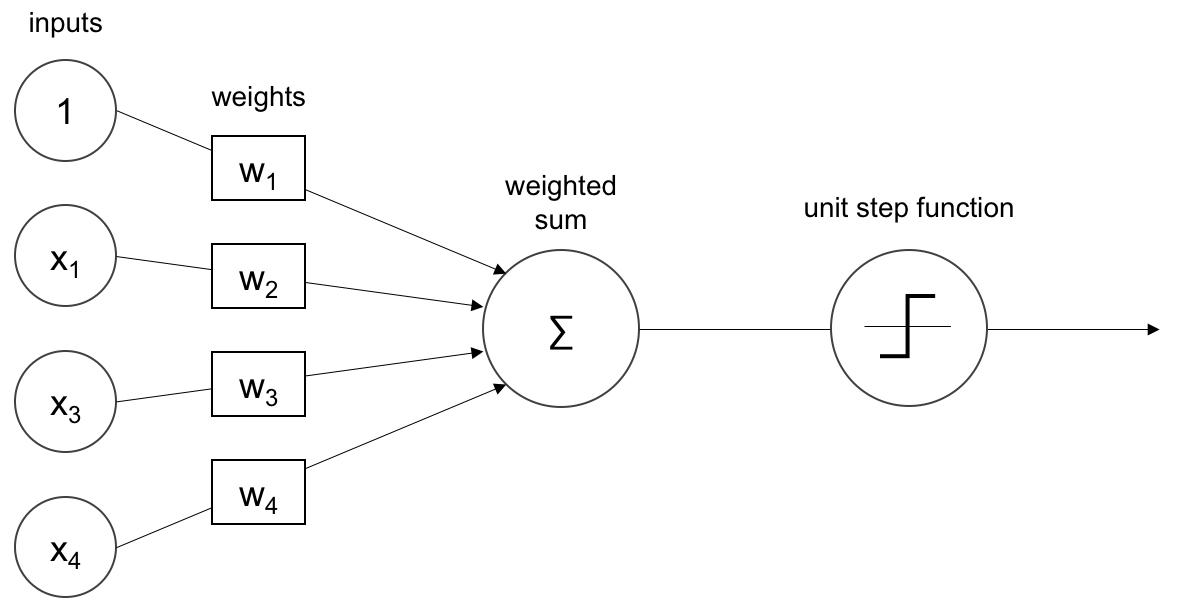
\includegraphics[width = 1 \textwidth]{Neural_Network/perceptron_schema.png}
           \caption{Schema of the Perceptron neuron}
       \end{center} 
    \end{minipage}
    \hspace{1em}
    \begin{minipage}{5cm}
        This Neural Network is formed by elements (the artificial neurons) called \textit{Perceptrons}. This neuron is formed by input, weight and activation functions.\\
        Nevertheless, the most important part of the neuron, and that determines significantly the capabilities of the neuron, is the activation function (which returns the output of the neuron).\\
    \end{minipage}
\end{figure}\\
The traditional activation function used in the Multilayer Perceptron is the Sigmoid: 
$$f(x) = \frac{1}{1+e^{-w\cdot x}},\text{ where: } x,w\in\mathbb{R}^n$$
The Multilayer Perceptron Topology can be splitted into layers of three types:
\begin{figure}[h]
    \begin{minipage}{9cm}
        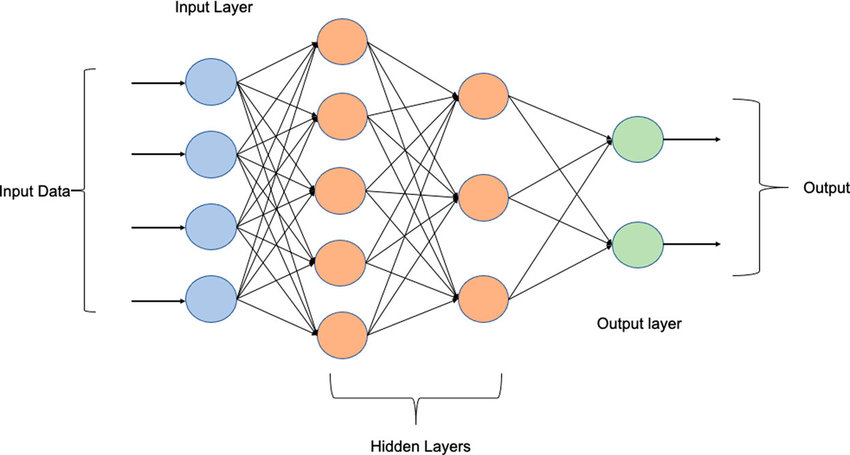
\includegraphics[width = 1 \textwidth]{Neural_Network/Multi-layer-perceptron-MLP-NN-basic-Architecture.png}
        \caption{Schema of the Multilayer perceptron}
    \end{minipage}
    \hspace{1em}
    \begin{minipage}{5cm}
        \begin{itemize}
            \item \textbf{Input Layer}: The initial set of neurons of the Multilayer Perceptron.
            \item \textbf{Output Layer}: The final set of neurons of the Multilayer Perceptron.
            \item \textbf{Hidden Layers}: The set of neurons (in layers) between the input and output layers.
        \end{itemize}
    \end{minipage}
\end{figure}\\
\newpage






% WHY WORKS
\subsection{Why Neural Networks works}
It is important to remark that what gives the capacity of model any system is because we can express everyproblem as a function (no matter if its a classification tasck, probability function, or prediction, regression function).\\
The association between a tasck and a function allow to apply the \textbf{Universal Approximation Theorem}.\\
\hline
\begin{itemize}
    \item \textbf{Definition:} Universal Approximation Theorem.
\end{itemize}  
For any function $f:\mathbb{R}^n \rightarrow \mathbb{R}^m$ and a subset $D\subset \mathbb{R}^n$ where $f$ is continuous at all $D$, 
$\exists \{(w_i, b_i, c_i)\}_{i = 0}^k$ that: 
$$f(\vec{x}) - \lim_{k \rightarrow \infty} \sum_{i=0}^{k} c_i \sigma \left( w^T \cdot \vec{x} + b_i \right) = 0$$
Where $w_i \in \mathbb{R}^n$, $b_i\in \mathbb{R}$, $c_i \in \mathbb{R}^m$, $\vec{x}\in D$ and $\sigma$ the sigmoid function.\\
\hline


\begin{thebibliography}{X}
\bibitem{WIKIPEDIA-MLP} \textsc{Wikipedia},
\textit{Multilayer perceptron},\\ \url{https://en.wikipedia.org/wiki/Multilayer_perceptron}
\bibitem{WIKIPEDIA-PERCERPTRON} \textsc{Wikipedia},
\textit{Perceptrón},\\ \url{https://es.wikipedia.org/wiki/Perceptr%C3%B3n}
\bibitem{WIKIPEDIA-ACTIV.FUNCT,} \textsc{Wikipedia},
\textit{Activation function},\\ \url{https://en.wikipedia.org/wiki/Activation_function}
\bibitem{WIKIPEDIA-FRANK} \textsc{Wikipedia},
\textit{Frank Rosenblatt},\\ \url{https://es.wikipedia.org/wiki/Frank_Rosenblatt}
\bibitem{WIKIPEDIA-ACTIVATINGFUNCTION} \textsc{Wikipedia},
\textit{Activating Function},\\ \url{https://en.wikipedia.org/wiki/Activating_function}
\bibitem{WIKIPEDIA-ART.NN} \textsc{Wikipedia},
\textit{Artificial neural network},\\ \url{https://en.wikipedia.org/wiki/Artificial_neural_network}
\bibitem{WIKIPEDIA-NN} \textsc{Wikipedia},
\textit{Neural network},\\ \url{https://en.wikipedia.org/wiki/Neural_network}
\bibitem{WIKIPEDIA-SIGMOID_TEOREM} \textsc{Wikipedia},
\textit{Universal Approximation Theorem},\\ \url{https://en.wikipedia.org/wiki/Universal_approximation_theorem}
\bibitem{WIKIPEDIA-MSE} \textsc{Wikipedia},
\textit{Mean Squared Error},\\ \url{https://en.wikipedia.org/wiki/Mean_squared_error}
\bibitem{WIKIPEDIA-MAE} \textsc{Wikipedia},
\textit{Mean Absolute Error},\\ \url{https://en.wikipedia.org/wiki/Mean_absolute_error}
\bibitem{WIKIPEDIA-CE} \textsc{Wikipedia},
\textit{Cross-Entropy},\\ \url{https://en.wikipedia.org/wiki/Cross-entropy}
\bibitem{WIKIPEDIA-BACKPROP} \textsc{Wikipedia},
\textit{BackPropagation},\\ \url{https://en.wikipedia.org/wiki/Backpropagation}

\bibitem{Dan} \textsc{Dantzig, G.B.} y \textsc{P. Wolfe},
<<Decomposition principle for linear programs>>,
\textit{Operations Research}, \textbf{8}, págs. 101--111, 1960.

\end{thebibliography}
\end{document}
